\documentclass[tikz,border=2pt]{standalone}
\usepackage{tikz}
\usetikzlibrary{shadows,decorations.pathmorphing}

\begin{document}
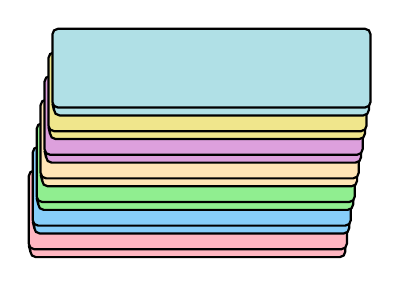
\begin{tikzpicture}
  % Define tray colors
  \definecolor{trayblue}{RGB}{135,206,250}
  \definecolor{traygreen}{RGB}{144,238,144}
  \definecolor{traypink}{RGB}{255,182,193}

\definecolor{tray1}{RGB}{255,182,193}  % Light Pink
\definecolor{tray2}{RGB}{135,206,250}  % Light Blue
\definecolor{tray3}{RGB}{144,238,144}  % Light Green
\definecolor{tray4}{RGB}{255,228,181}  % Moccasin
\definecolor{tray5}{RGB}{221,160,221}  % Plum
\definecolor{tray6}{RGB}{240,230,140}  % Khaki
\definecolor{tray7}{RGB}{176,224,230}  % Powder Blue
\definecolor{tray8}{RGB}{255,160,122}  % Light Salmon
\definecolor{tray9}{RGB}{152,251,152}  % Pale Green
\definecolor{tray10}{RGB}{255,222,173} % Navajo White


  % Draw trays in a stack
  \foreach \i/\color in {0/tray1,1/tray2,2/tray3,3/tray4,4/tray5,5/tray6,6/tray7} {
    \begin{scope}[yshift=\i*0.3cm, xshift=\i*0.05cm]
      \draw[fill=\color, thick, rounded corners=2pt]
        (0,0) rectangle (4,1);
      \draw[fill=\color, thick, rounded corners=2pt]
        (-0.02,0.1) rectangle (4.02,1.1);
      \draw[thick]
        (0,2pt) -- (-0.02,0.15);
    %   % Add cartoon-style squiggle
    %   \draw[decorate, decoration={zigzag,segment length=4,amplitude=1}, thick]
    %     (0,1) -- (4,1);
    \end{scope}
  }

%   % Optional: Add a label
%   \node[font=\large\sffamily, align=center] at (2,3.2) {Cartoon Tray Stack};
\end{tikzpicture}
\end{document}